%%%%%%%%%%%%%%%%%%%%%%%%%%%%%%%%%%%%%%
%%%%%%%%%%%%%%%%%%%%%%%%%%%%%%%%%%%%%%
% Do not edit the TeX file your work
% will be overwritten.  Edit the RnW
% file instead.
%%%%%%%%%%%%%%%%%%%%%%%%%%%%%%%%%%%%%%
%%%%%%%%%%%%%%%%%%%%%%%%%%%%%%%%%%%%%%




\newcommand{\FunctionPathsMultFig}{

\begin{knitrout}
\definecolor{shadecolor}{rgb}{0.969, 0.969, 0.969}\color{fgcolor}\begin{figure}[!h]

{\centering 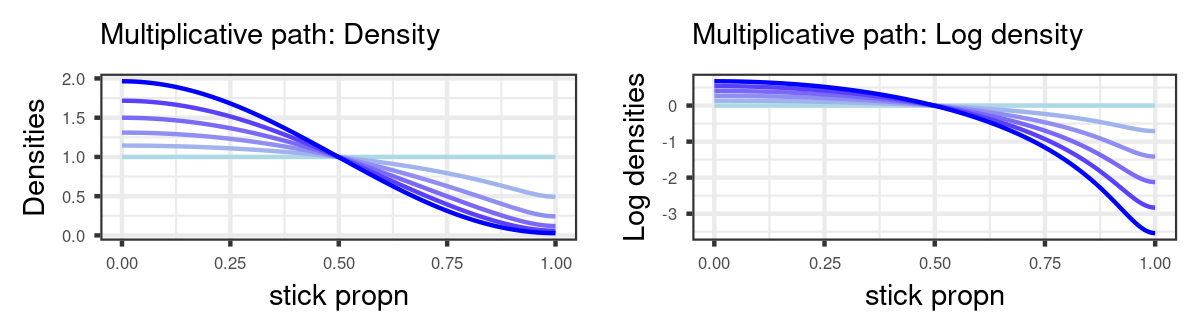
\includegraphics[width=0.980\linewidth,height=0.274\linewidth]{figure/mult_path-1} 

}

\caption[Multiplicative mixture paths between two densities]{Multiplicative mixture paths between two densities.}\label{fig:mult_path}
\end{figure}


\end{knitrout}
}


\newcommand{\FunctionPathsLinFig}{

\begin{knitrout}
\definecolor{shadecolor}{rgb}{0.969, 0.969, 0.969}\color{fgcolor}\begin{figure}[!h]

{\centering 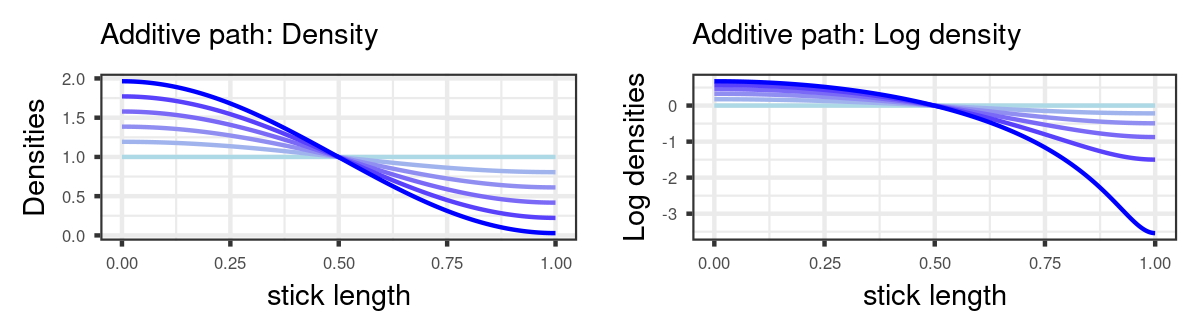
\includegraphics[width=0.980\linewidth,height=0.274\linewidth]{figure/lin_path-1} 

}

\caption[Linear mixture paths between two densities]{Linear mixture paths between two densities.}\label{fig:lin_path}
\end{figure}


\end{knitrout}
}


\newcommand{\FunctionBallFig}{

\begin{knitrout}
\definecolor{shadecolor}{rgb}{0.969, 0.969, 0.969}\color{fgcolor}\begin{figure}[!h]

{\centering 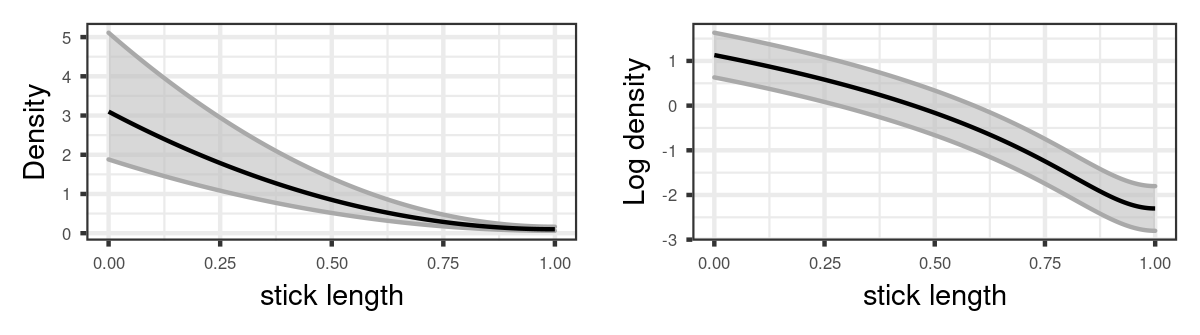
\includegraphics[width=0.980\linewidth,height=0.274\linewidth]{figure/func_ball-1} 

}

\caption[An $\linf{\cdot}$ ball]{An $\linf{\cdot}$ ball.}\label{fig:func_ball}
\end{figure}


\end{knitrout}
}
